\section{Results}
\label{sec:results}

\begin{table}[t]
\floatconts{tab:main}
{\caption{F1 on the unseen scanner (mean over 10 student seeds, then over the three held-out scanners; 95\% interval from
a paired bootstrap over images and seeds). Each student uses its own teacher for TGR. --: not applicable (ConvNeXt-T has
no BatchNorm) or not run. Last row: (student $-$ no-teacher student) / (teacher $-$ no-teacher student).
$^\dagger$UNI's advantage over the no-teacher student is only 0.055 F1, so its share is unstable; its seed-0 LoRA
teacher chose an unusually low cutoff on the source scanners.}}
{%
\scriptsize
\setlength{\tabcolsep}{3pt}
\begin{tabular}{@{}lcccc@{\hspace{8pt}}cc@{}}
\toprule
 & \multicolumn{4}{c}{ResNet-18 student (11 M)} & \multicolumn{2}{c}{ConvNeXt-T student (28 M)} \\
\cmidrule(lr){2-5}\cmidrule(l){6-7}
Teacher & H-optimus-0 & Virchow2 & UNI2-h & UNI & H-optimus-0 & Virchow2 \\
\midrule
No-teacher student & \makecell{0.711\\{\scriptsize[.682, .735]}} & \makecell{0.711\\{\scriptsize[.682, .735]}} & \makecell{0.711\\{\scriptsize[.682, .735]}} & \makecell{0.711\\{\scriptsize[.682, .735]}} & \makecell{0.736\\{\scriptsize[.708, .759]}} & \makecell{0.736\\{\scriptsize[.708, .759]}} \\
Distillation (KD) & \makecell{0.725\\{\scriptsize[.696, .748]}} & \makecell{0.722\\{\scriptsize[.694, .744]}} & \makecell{0.704\\{\scriptsize[.673, .729]}} & \makecell{0.716\\{\scriptsize[.685, .741]}} & \makecell{0.765\\{\scriptsize[.740, .785]}} & \makecell{0.761\\{\scriptsize[.736, .781]}} \\
\quad + TGR & \makecell{0.762\\{\scriptsize[.739, .779]}} & \makecell{0.748\\{\scriptsize[.724, .767]}} & \makecell{0.744\\{\scriptsize[.720, .762]}} & \makecell{0.720\\{\scriptsize[.693, .741]}} & \makecell{0.801\\{\scriptsize[.781, .817]}} & \makecell{0.789\\{\scriptsize[.768, .806]}} \\
\quad + AdaBN + TGR & \makecell{0.777\\{\scriptsize[.752, .796]}} & \makecell{0.775\\{\scriptsize[.750, .793]}} & \makecell{0.768\\{\scriptsize[.745, .786]}} & \makecell{0.738\\{\scriptsize[.709, .759]}} & -- & -- \\
KD + TGA (retrained) & \makecell{0.788\\{\scriptsize[.768, .805]}} & \makecell{0.781\\{\scriptsize[.760, .798]}} & \makecell{0.771\\{\scriptsize[.750, .789]}} & \makecell{0.782\\{\scriptsize[.761, .799]}} & \makecell{0.805\\{\scriptsize[.784, .822]}} & \makecell{0.805\\{\scriptsize[.785, .821]}} \\
No-teacher adaptation & \makecell{0.769\\{\scriptsize[.744, .788]}} & \makecell{0.769\\{\scriptsize[.744, .788]}} & \makecell{0.769\\{\scriptsize[.744, .788]}} & \makecell{0.769\\{\scriptsize[.744, .788]}} & \makecell{0.775\\{\scriptsize[.749, .795]}} & \makecell{0.775\\{\scriptsize[.749, .795]}} \\
Teacher (seed 0) & \makecell{0.814\\{\scriptsize[.794, .830]}} & \makecell{0.805\\{\scriptsize[.785, .822]}} & \makecell{0.797\\{\scriptsize[.776, .813]}} & \makecell{0.767\\{\scriptsize[.743, .785]}} & \makecell{0.814\\{\scriptsize[.794, .830]}} & \makecell{0.805\\{\scriptsize[.785, .822]}} \\
\midrule
Share recovered by KD + TGA & \makecell{75\%\\{\scriptsize[64, 85]}} & \makecell{74\%\\{\scriptsize[62, 87]}} & \makecell{70\%\\{\scriptsize[54, 85]}} & \makecell{128\%$^\dagger$\\{\scriptsize[106, 174]}} & \makecell{88\%\\{\scriptsize[74, 104]}} & \makecell{99\%\\{\scriptsize[83, 121]}} \\
\bottomrule
\end{tabular}
}
\end{table}


\subsection{RQ1: distillation transfers ranking, not robustness}

The LoRA teachers reach a new-scanner F1 of 0.767 to 0.814 (\tableref{tab:main}; means over three LoRA seeds 0.778 to
0.812, in line with \citealp{ammeling2026benchmarking}); the no-teacher ResNet-18 student reaches 0.711. Yet distilling any of the four teachers into ResNet-18 changes its F1 by only $-0.007$ to $+0.013$,
and every 95\% interval includes zero. ConvNeXt-T benefits more (+0.029, +0.014 to +0.045, with H-optimus-0; +0.025
with Virchow2) but recovers only 37\% and 36\% of the teacher's advantage (48\% and 63\% with two other
trainings of H-optimus-0). The shortfall is not a failure to rank cells: the AUROC of the distilled ResNet-18
students (0.879 to 0.894) exceeds that of the no-teacher student (0.872) and follows the teachers' order, so the loss in
F1 lies elsewhere.

\subsection{RQ2: where the gap sits depends on the student}

\begin{figure}[t]
\floatconts
  {fig:gap}
  {\caption{Where the gap sits. Each bar splits the teacher's advantage over the no-teacher student (0\% to 100\%) into
  distillation, operating point (TGR), normalisation statistics (AdaBN; Shapley credit over the two post-hoc layers),
  retraining (TGA beyond the post-hoc layers) and the remaining gap; triangles: retrained student with 95\% interval.
  UNI's advantage is too small for a stable share (\tableref{tab:main}).}}
  {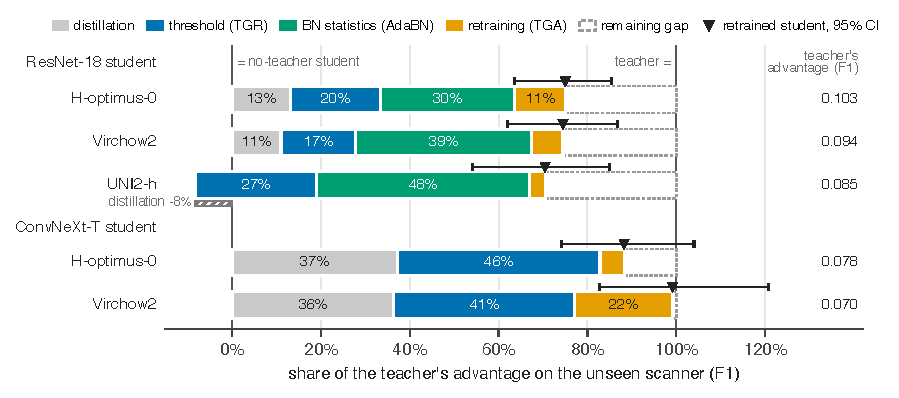
\includegraphics[width=\linewidth]{figures/fig2_where_the_gap_sits}}
\end{figure}

For the ResNet-18 student, the two post-hoc layers recover most of the teacher's advantage without retraining
(\figureref{fig:gap}): the operating point accounts for 17\% to 27\% and the BatchNorm statistics for 30\% to 48\%,
together 51\% to 75\% for the three teachers with a reliable operating point. Once both are repaired, retraining adds
only 4\% to 11\%, and 25\% to 30\% remains. ConvNeXt-T, by contrast, has no statistics to re-estimate; there the
operating point alone accounts for 46\% (H-optimus-0) and 41\% (Virchow2), and retraining adds 5\% and 22\%. Retraining is not AdaBN in disguise: putting source
statistics back into the retrained ResNet-18 student costs only 0.011 (S360) and 0.007 F1 (XR)
(Appendix~\ref{app:ladder}).

\subsection{RQ3a: the operating point needs the teacher, but only a few images of it}
\label{sec:res-threshold}

\begin{figure}[t]
\floatconts
  {fig:threshold}
  {\caption{The operating point. (a, b) F1 against the number of new-scanner images per half, used unlabelled (TGR,
  AdaBN) or labelled (labelled cutoff); means over folds, seeds and 10 image draws, bands: range over draws. (c, d) F1
  after resampling new-scanner cells to a given mitosis prevalence; grey: source prevalence range.}}
  {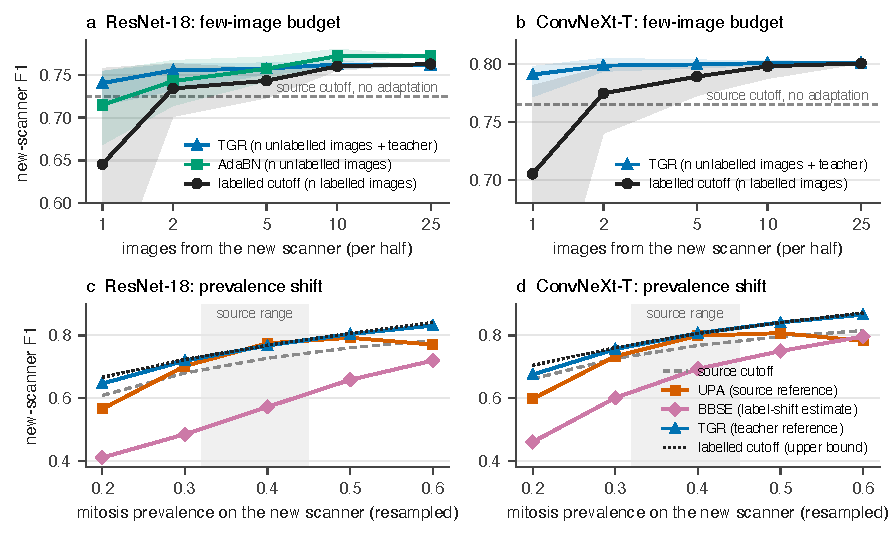
\includegraphics[width=0.95\linewidth]{figures/fig3_threshold_layer}}
\end{figure}

One teacher-referenced offset closes the threshold gap from few images: TGR brings both KD students to the bound of a cutoff chosen with the new scanner's labels (ResNet-18: 0.762 vs.\
0.762; ConvNeXt-T: 0.801 vs.\ 0.800), +0.037 (+0.022 to +0.053) and +0.036 (+0.022 to +0.052) over the source cutoff
(Holm $p<0.001$), and it comes within 0.005 of that bound from five unlabelled images per half on
(\figureref{fig:threshold}a,b). With a single image it beats AdaBN, whose statistics cannot be estimated from so few
cells (+0.025, +0.010 to +0.041, Holm $p=0.004$), and at every budget it matches or beats a cutoff chosen from the labels
of the same images (one image: 0.740 vs.\ 0.646; Appendix~\ref{app:few}).

What the teacher contributes here is the target prevalence. At the natural prevalence, close to that of the source
scanners, keeping the source positive rate (what UPA reduces to at one operating point) is only 0.002 below TGR for ResNet-18 ($-0.008$ to $+0.012$, contrary to our expectation) and 0.019
below for ConvNeXt-T (+0.009 to +0.031, Holm $p<0.001$). Once the prevalence changes, however, source-referenced
methods break while TGR stays near the labelled bound (\figureref{fig:threshold}c,d): at 0.2 or 0.6 it beats the source positive rate by 0.061 to 0.083 (four pre-specified contrasts, Holm $p<0.001$) and the same
offset referenced to the source mean probability by 0.025 to 0.126. Three other teacher-referenced recalibrations stay
within 0.015 of TGR (Appendix~\ref{app:baselines}), so the reference matters more than the functional form. Prior-shift
estimators, conversely, fail even at the natural prevalence (EM, EM with bias-corrected calibration, BBSE: 0.52 to 0.55
for ResNet-18): on S360 the student calls 21\% of cells positive (true prevalence 35\%) and they conclude 4\% to 9\%,
reading the scanner-induced score shift as a prevalence change.

\subsection{RQ3b: retraining gains come mostly from the unlabelled images}

Retraining with the teacher on the unlabelled half (TGA) is the largest step: +0.060 to +0.067 over the KD
ResNet-18 student for every teacher (Holm $p<0.001$), and +0.040 (H-optimus-0) and +0.044 (Virchow2, Holm $p<0.001$)
for ConvNeXt-T. Most of this gain, however, does not need the teacher. For ResNet-18, the target images alone reach 75\% to 96\% of TGA's gain over the no-teacher student (0.769),
and the teacher adds +0.002 to +0.019 (not significant after Holm correction for the three pre-specified teachers;
+0.019, +0.006 to +0.034, for H-optimus-0, analysed before the protocols were written). AdaBN, TENT and TGR together
reach 0.784 without retraining, 0.005 ($-0.005$ to $+0.016$) below TGA. For ConvNeXt-T, the target images alone still
reach most of TGA's gain, 57\% (34\% to 76\%; 0.775), but the teacher adds a significant +0.030 with both teachers (+0.016 to +0.045 and +0.017 to +0.046, Holm
$p<0.001$). Here the adapted no-teacher student even stays below KD + TGR without retraining ($-0.025$, $-0.014$;
descriptive), perhaps limited by its ResNet-18 pseudo-labels.

\subsection{RQ4: a student 23--41 times smaller close to its teacher}

\begin{figure}[t]
\floatconts
  {fig:close}
  {\caption{How close and how cheap. Left: student minus the teacher training it was distilled from (LoRA seed 0 unless
  stated), F1 with 95\% intervals; filled: pre-specified (margin $-0.02$, dashed; brown: mean of three trainings);
  open: descriptive. Right: throughput.}}
  {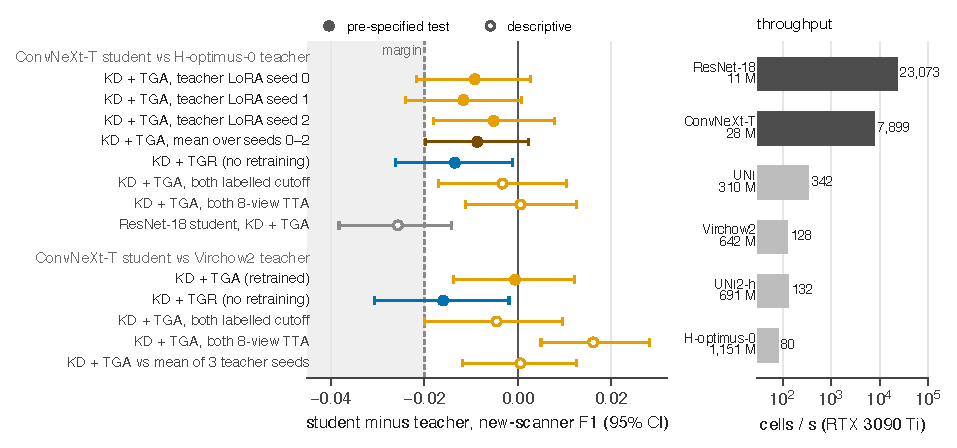
\includegraphics[width=0.95\linewidth]{figures/fig4_close_and_cheap}}
\end{figure}

Repaired in all three layers, the ConvNeXt-T student recovers 88\% (74\% to 104\%)
of H-optimus-0's advantage and 99\% (83\% to 121\%) of Virchow2's. It is non-inferior to Virchow2 at the pre-specified
margin ($-0.001$, $-0.014$ to $+0.012$; Holm $p=0.004$). Against H-optimus-0 it is 0.009 lower ($-0.022$ to $+0.003$),
so non-inferiority is not established ($p=0.085$; \figureref{fig:close}), nor for students of two other LoRA
trainings of this teacher (pre-specified, Appendix~\ref{app:fc}): they recover 86\% and 92\% of their own teacher's
advantage and stay 0.012 ($-0.024$ to $+0.001$) and 0.005 ($-0.018$ to $+0.008$) below it (Holm $p=0.090$ and
$0.027$; we expected non-inferiority for seed 2). On average over the three trainings the gap is 0.009 (lower limit
$-0.0198$), half the spread of the teacher's own F1 across them (0.020). With TGR alone, the KD
students stay below both seed-0 teachers ($-0.013$, $-0.016$), and the retrained ResNet-18 student remains 0.026
($-0.038$ to $-0.014$) below H-optimus-0. Neither the operating point nor test-time augmentation explains the comparison: with labelled cutoffs on both sides
the differences are $-0.003$ (H-optimus-0) and $-0.004$ (Virchow2), and eight-view augmentation does not help the
teachers (0.814 to 0.812; 0.805 to 0.797). With 23 to 41 times fewer parameters, the
ConvNeXt-T student classifies 7{,}899 cells per second, 62 and 98 times as many as Virchow2 and H-optimus-0 (8 to 12
times if only the student uses eight-view augmentation), and the teacher is needed only once per new scanner.
